
\documentclass[border=10pt, 12pt]{standalone}
\usepackage[svgnames]{xcolor}
\usepackage{amsmath}
\usepackage{pgfplots}
\pgfplotsset{compat=newest}
\usepackage[sfdefault]{FiraSans}
\usepackage{FiraMono}
\renewcommand*\familydefault{\sfdefault}
\begin{document}
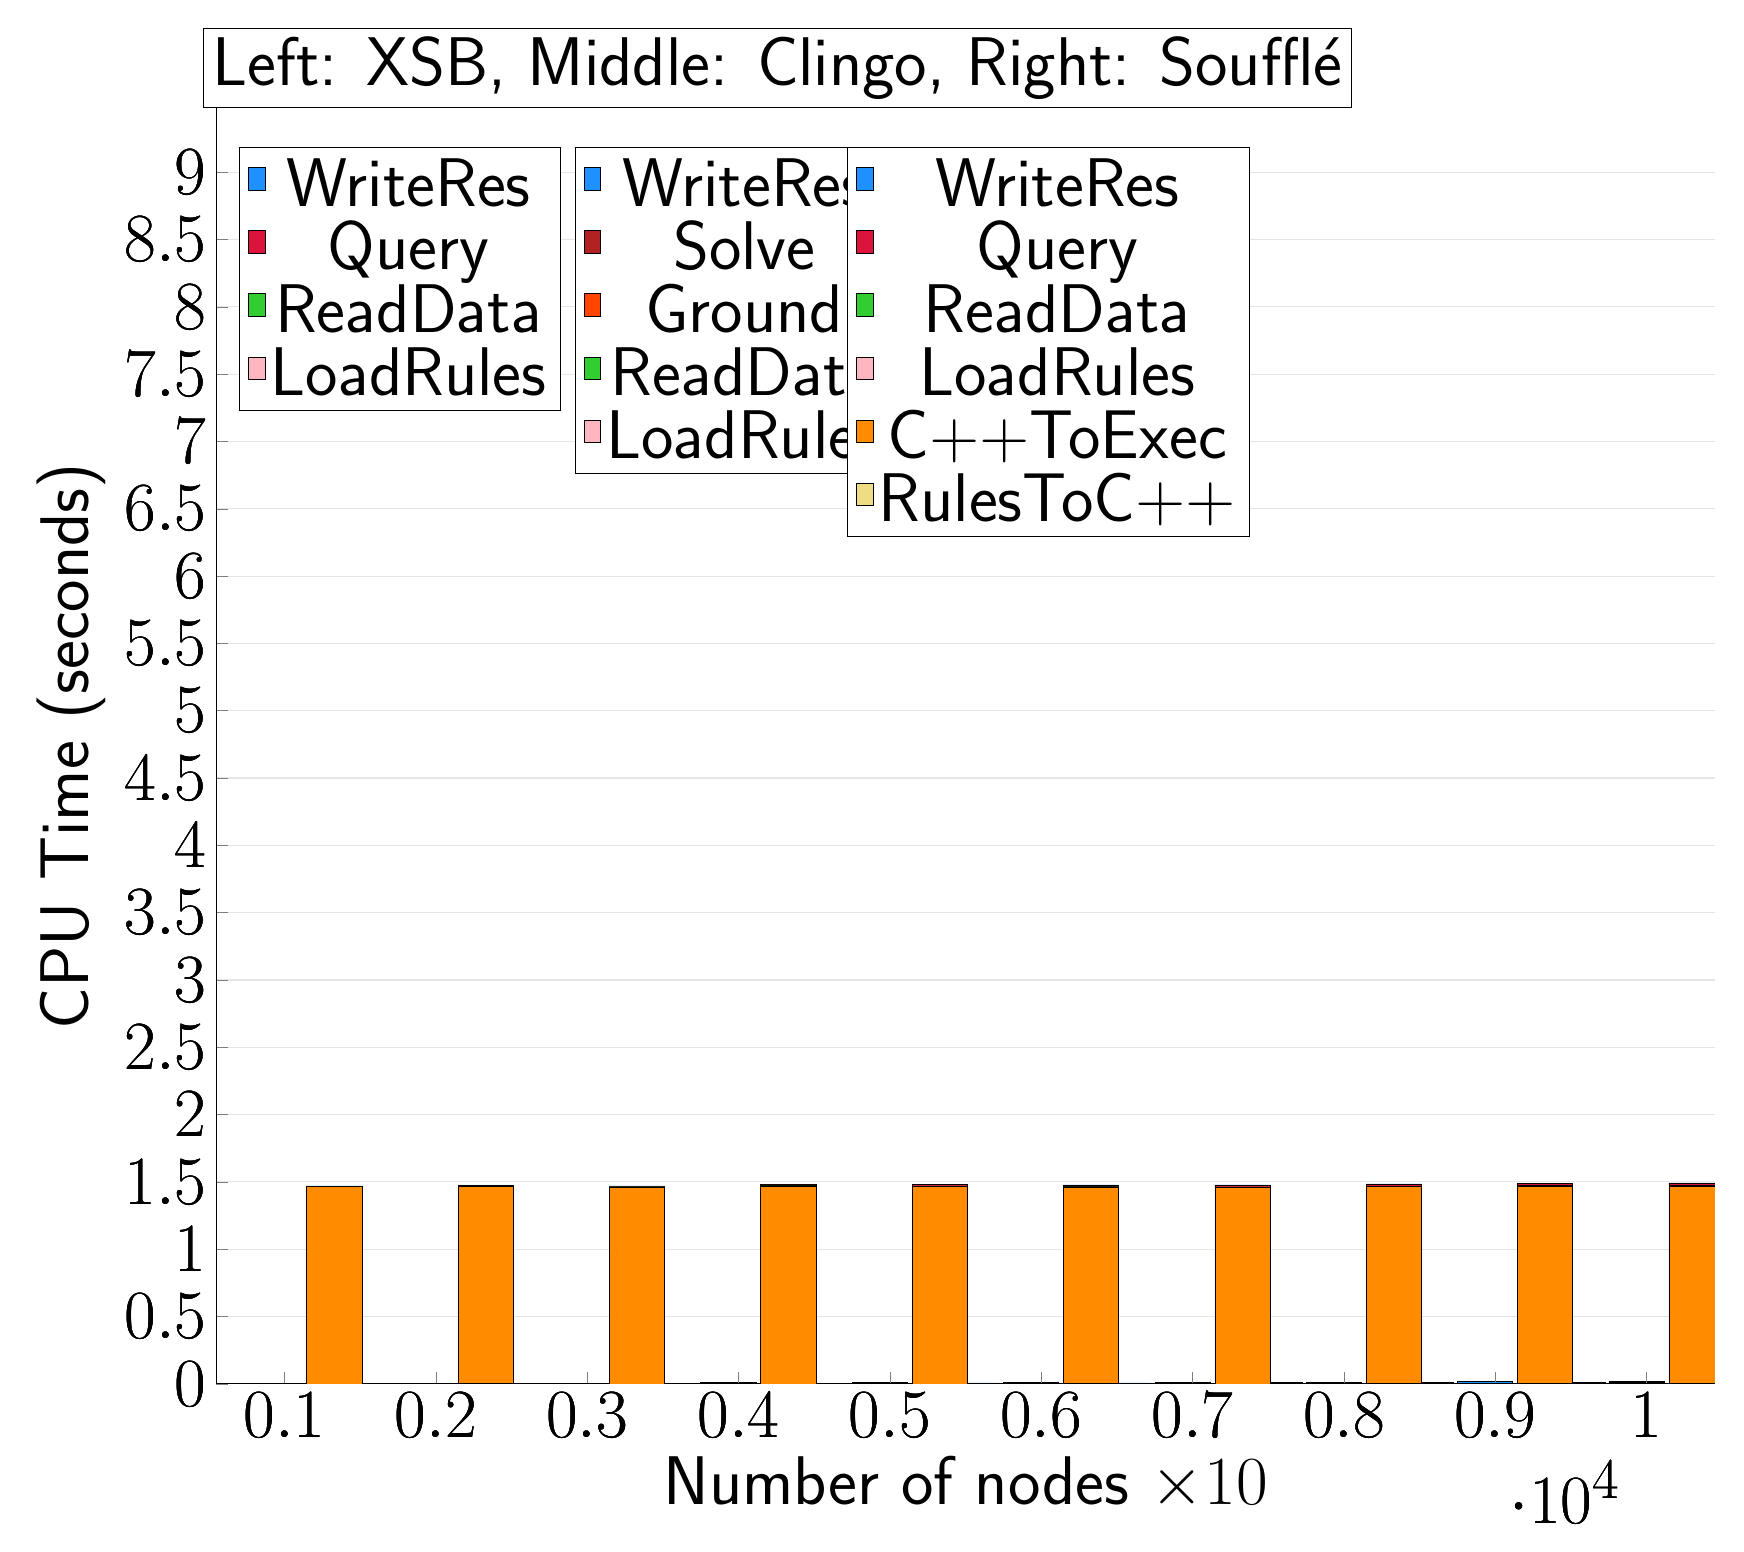
\begin{tikzpicture}
                        \begin{axis}[bar shift=-25pt, 
   ybar stacked,
   width=1.7\textwidth,
   bar width=0.7cm,
   ymajorgrids, tick align=inside,
   major grid style={draw=gray!20},
   xtick=data,
   ymin=0, ymax=9.474,
   axis x line*=bottom,
   axis y line*=left,
   enlarge x limits=0.05,
   legend style={
       at={(0.23, 0.97)},
       anchor=north east,
       legend columns=1,
       font=\Huge,
   },
   ylabel={CPU Time (seconds)},
   xlabel={Number of nodes $\times 10$},
   label style={font=\Huge},
   tick label style={font=\Huge},
]
\addlegendimage{fill=DodgerBlue, draw=black, line width=0.2pt}
\addlegendentry{WriteRes}
\addlegendimage{fill=Crimson, draw=black, line width=0.2pt}
\addlegendentry{Query}
\addlegendimage{fill=LimeGreen, draw=black, line width=0.2pt}
\addlegendentry{ReadData}
\addlegendimage{fill=LightPink, draw=black, line width=0.2pt}
\addlegendentry{LoadRules}
\addplot +[fill=LightPink, draw=black, line width=0.2pt] coordinates {
(1000, 0.0005488)
(2000, 0.0005468000000000002)
(3000, 0.0005482)
(4000, 0.0005479999999999998)
(5000, 0.0005490000000000002)
(6000, 0.0005473999999999998)
(7000, 0.0005560000000000003)
(8000, 0.000548599999999999)
(9000, 0.0005493999999999994)
(10000, 0.0005520000000000002)
};
\addplot +[fill=LimeGreen, draw=black, line width=0.2pt] coordinates {
(1000, 0.0002048000000000002)
(2000, 0.0002838)
(3000, 0.0003615999999999998)
(4000, 0.00043880000000000004)
(5000, 0.0005191999999999996)
(6000, 0.0005995999999999999)
(7000, 0.0006732)
(8000, 0.0007496000000000002)
(9000, 0.000828)
(10000, 0.0009295999999999998)
};
\addplot +[fill=Crimson, draw=black, line width=0.2pt] coordinates {
(1000, 7.500000000000003e-05)
(2000, 0.00013780000000000002)
(3000, 0.0001960000000000002)
(4000, 0.0002568000000000002)
(5000, 0.00031260000000000044)
(6000, 0.00037240000000000027)
(7000, 0.0004236000000000002)
(8000, 0.00048159999999999956)
(9000, 0.0005412000000000001)
(10000, 0.000595)
};
\addplot +[fill=DodgerBlue, draw=black, line width=0.2pt] coordinates {
(1000, 0.0009450000000000002)
(2000, 0.0017749999999999999)
(3000, 0.0025957999999999997)
(4000, 0.0034431999999999996)
(5000, 0.004286999999999999)
(6000, 0.0050816)
(7000, 0.0059374)
(8000, 0.0067694)
(9000, 0.007615799999999999)
(10000, 0.0085106)
};
\end{axis}

\begin{axis}[bar shift=-3.7pt, 
   ybar stacked,
   width=1.7\textwidth,
   bar width=0.7cm,
   ymajorgrids, tick align=inside,
   major grid style={draw=none},
   xtick=data,
   ymin=0, ymax=9.474,
   axis x line*=none,
   axis y line*=none,
   enlarge x limits=0.05,
   legend style={
       at={(0.454, 0.97)},
       anchor=north east,
       legend columns=1,
       font=\Huge,
   },
   label style={font=\Huge},
   tick label style={font=\Huge},
]
\addlegendimage{fill=DodgerBlue, draw=black, line width=0.2pt}
\addlegendentry{WriteRes}
\addlegendimage{fill=FireBrick, draw=black, line width=0.2pt}
\addlegendentry{Solve}
\addlegendimage{fill=OrangeRed, draw=black, line width=0.2pt}
\addlegendentry{Ground}
\addlegendimage{fill=LimeGreen, draw=black, line width=0.2pt}
\addlegendentry{ReadData}
\addlegendimage{fill=LightPink, draw=black, line width=0.2pt}
\addlegendentry{LoadRules}
\addplot +[fill=LightPink, draw=black, line width=0.2pt] coordinates {
(1000, 0.0)
(2000, 0.0)
(3000, 0.0)
(4000, 0.0)
(5000, 0.0)
(6000, 0.0)
(7000, 0.0)
(8000, 0.0)
(9000, 0.0)
(10000, 0.0)
};
\addplot +[fill=LimeGreen, draw=black, line width=0.2pt] coordinates {
(1000, 0.0)
(2000, 0.0)
(3000, 0.0)
(4000, 0.0)
(5000, 0.0)
(6000, 0.0)
(7000, 0.0)
(8000, 0.0)
(9000, 0.0)
(10000, 0.0)
};
\addplot +[fill=OrangeRed, draw=black, line width=0.2pt] coordinates {
(1000, 0.0)
(2000, 0.0)
(3000, 0.0)
(4000, 0.0)
(5000, 0.0)
(6000, 0.0)
(7000, 0.0)
(8000, 0.0020000000000000018)
(9000, 0.0040000000000000036)
(10000, 0.006000000000000005)
};
\addplot +[fill=FireBrick, draw=black, line width=0.2pt] coordinates {
(1000, 0.0)
(2000, 0.0)
(3000, 0.0)
(4000, 0.0)
(5000, 0.0)
(6000, 0.0)
(7000, 0.0)
(8000, 0.0020000000000000018)
(9000, 0.0)
(10000, 0.0040000000000000036)
};
\addplot +[fill=DodgerBlue, draw=black, line width=0.2pt] coordinates {
(1000, 0.0)
(2000, 0.0)
(3000, 0.0)
(4000, 0.010000000000000009)
(5000, 0.010000000000000009)
(6000, 0.010000000000000009)
(7000, 0.010000000000000009)
(8000, 0.008000000000000007)
(9000, 0.016000000000000014)
(10000, 0.006000000000000005)
};
\end{axis}

\begin{axis}[bar shift=18pt, 
   ybar stacked,
   width=1.7\textwidth,
   bar width=0.7cm,
   ymajorgrids, tick align=inside,
   major grid style={draw=none},
   xtick=data,
   ymin=0, ymax=9.474,
   axis x line*=none,
   axis y line*=none,
   enlarge x limits=0.05,
   legend style={
       at={(0.69, 0.97)},
       anchor=north east,
       legend columns=1,
       font=\Huge,
   },
   label style={font=\Huge},
   tick label style={font=\Huge},
]
\addlegendimage{fill=DodgerBlue, draw=black, line width=0.2pt}
\addlegendentry{WriteRes}
\addlegendimage{fill=Crimson, draw=black, line width=0.2pt}
\addlegendentry{Query}
\addlegendimage{fill=LimeGreen, draw=black, line width=0.2pt}
\addlegendentry{ReadData}
\addlegendimage{fill=LightPink, draw=black, line width=0.2pt}
\addlegendentry{LoadRules}
\addlegendimage{fill=DarkOrange, draw=black, line width=0.2pt}
\addlegendentry{C++ToExec}
\addlegendimage{fill=LightGoldenrod, draw=black, line width=0.2pt}
\addlegendentry{RulesToC++}
\addplot +[fill=LightGoldenrod, draw=black, line width=0.2pt] coordinates {
(1000, 0.0)
(2000, 0.0020000000000000005)
(3000, 0.0)
(4000, 0.0)
(5000, 0.0)
(6000, 0.0020000000000000005)
(7000, 0.0)
(8000, 0.0020000000000000005)
(9000, 0.0020000000000000005)
(10000, 0.0020000000000000005)
};
\addplot +[fill=DarkOrange, draw=black, line width=0.2pt] coordinates {
(1000, 1.466)
(2000, 1.464)
(3000, 1.462)
(4000, 1.468)
(5000, 1.468)
(6000, 1.46)
(7000, 1.46)
(8000, 1.464)
(9000, 1.466)
(10000, 1.466)
};
\addplot +[fill=LightPink, draw=black, line width=0.2pt] coordinates {
(1000, 0.0001462)
(2000, 0.0001584)
(3000, 0.00015920000000000002)
(4000, 0.0001614)
(5000, 0.00016900000000000002)
(6000, 0.00015219999999999999)
(7000, 0.00016480000000000002)
(8000, 0.0001492)
(9000, 0.000161)
(10000, 0.00015460000000000002)
};
\addplot +[fill=LimeGreen, draw=black, line width=0.2pt] coordinates {
(1000, 0.0009195999999999999)
(2000, 0.001249)
(3000, 0.0013978)
(4000, 0.0020926)
(5000, 0.0025614)
(6000, 0.0027114)
(7000, 0.0030868)
(8000, 0.0032672)
(9000, 0.0036792000000000005)
(10000, 0.004202599999999999)
};
\addplot +[fill=Crimson, draw=black, line width=0.2pt] coordinates {
(1000, 0.0022612)
(2000, 0.003946)
(3000, 0.004704)
(4000, 0.007535)
(5000, 0.0088392)
(6000, 0.009482599999999999)
(7000, 0.0115186)
(8000, 0.012756599999999998)
(9000, 0.014303399999999999)
(10000, 0.0159078)
};
\addplot +[fill=DodgerBlue, draw=black, line width=0.2pt] coordinates {
(1000, 0.0012092000000000001)
(2000, 0.0017364000000000001)
(3000, 0.0017752)
(4000, 0.0021376000000000004)
(5000, 0.0029748000000000005)
(6000, 0.002987)
(7000, 0.003474)
(8000, 0.0037274)
(9000, 0.004065)
(10000, 0.0044800000000000005)
};
\end{axis}


\node[anchor=south, draw, fill=white] at (rel axis cs:0.42,1) {\Huge Left: XSB, Middle: Clingo, Right: Soufflé};
\end{tikzpicture}
\end{document}
                    